\section{Resultados y discusión}

\subsection{Análisis Cuantitativo}

\subsubsection{Objetivo:}

Realizamos dos pruebas del tiempo de cómputo necesario para resolver el problema del presente trabajo.
En el primero variamos la cantidad de páginas manteniendo una proporción de los links entre ellas.
En el segundo fijamos la cantidad de páginas y variamos la densidad de la misma.

epsilon: $10^{-9}$

Nodos: 500, 30 veces, 50 de distancia, porcentaje de ejes: 1, 10, 33. Repeticiones 5. 
     %500, 17 veces, 250 distancia, prop 15, rep 5
%viejos nodos: 500, 25, 100, 200 ejes fijo
\\
Ejes: Mantenemos la cantidad de nodos fijos en 1000, iteramos 25 desde $\frac{nodos \times nodos-1}{25}$ hasta $nodos \times nodos-1$ (es decir, dividimos la cantidad máxima de ejes que puede tener un grafo dirigido en 25 y en cada iteración le sumamos esa fracción hasta llegar al grafo completo), repitiendo el cálculo 5 veces y promediándo el tiempo reportado.

p: nodos 1000, ejes 8000, p = {0.1 ... 0.9} $\cup$ {0.85}. Repeticiones 5.

\subsubsection{Hipótesis:}

Cúbica en nodos, lineal en ejes. A medida que aumenta el p más costosa es la computación del PageRank.

\subsubsection{Resultado y Análisis: }

Comenzemos analizando el experimento sobre la cantidad de nodos:

         \noindent{} \begin{minipage}{\textwidth}
                \begin{center}
                    \vspace{1em}

                    \begin{tabular}{cc}
                        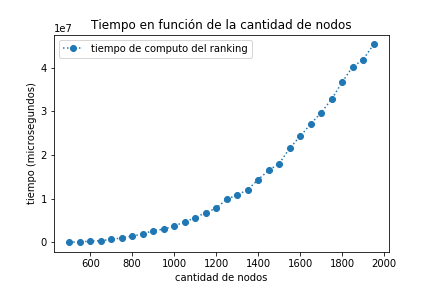
\includegraphics[width=0.475\textwidth]{img/tiempo_nodos_prop_500-2000_solo_e100.png}
                       & 
                        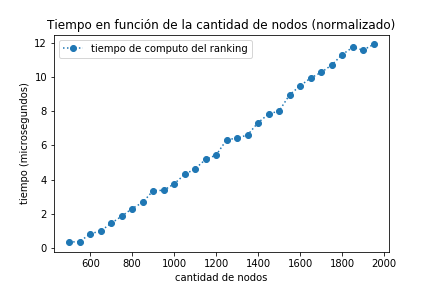
\includegraphics[width=0.475\textwidth]{img/tiempo_nodos_prop_500-2000-normalizado-e100.png}								\\
                        Con $1\%$ de ejes & Con $1\%$ de ejes normalizado por $x^{2}$ \\
                        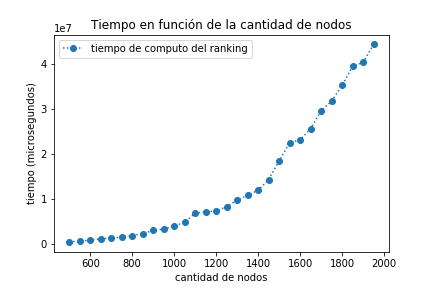
\includegraphics[width=0.475\textwidth]{img/tiempo_nodos_prop_500-2000_solo_e10.png} 
       & 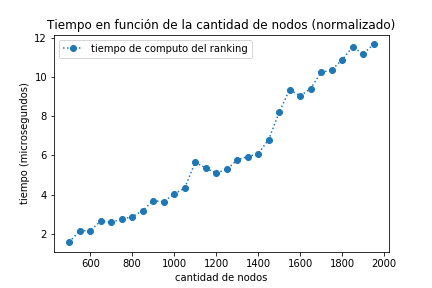
\includegraphics[width=0.475\textwidth]{img/tiempo_nodos_prop_500-2000-normalizado-e10.png} \\
             Con $10\%$ de ejes & Con $10\%$ de ejes normalizado por $x^{2}$ \\
      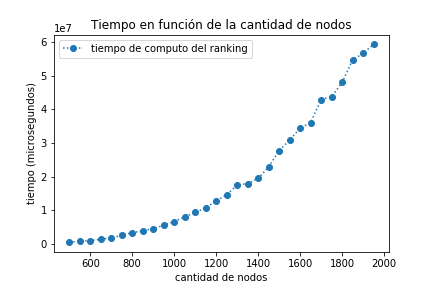
\includegraphics[width=0.475\textwidth]{img/tiempo_nodos_prop_500-2000_solo_e3.png} 
       & 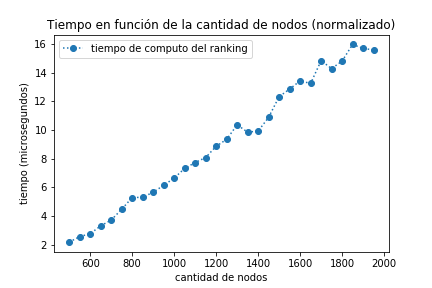
\includegraphics[width=0.475\textwidth]{img/tiempo_nodos_prop_500-2000-normalizado-e3.png} \\
             Con $33\%$ de ejes & Con $33\%$ de ejes normalizado por $x^{2}$ \\
                    \end{tabular}

                    \vspace{1em}

Resultado de la ejecución del algoritmo en función del cantidad de nodos para tres porcentajes de ejes diferentes. En las figuras de las derecha se lo normaliza por una función cuadrática.

                    \vspace{1em}
                \end{center}
                \label{fig:exp1-nodos}
            \end{minipage}




Por otro lado, la iteración sobre los ejes arrojó el siguiente resultado:

\begin{figure}
   \begin{center}
     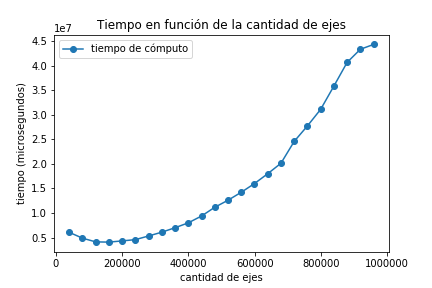
\includegraphics{img/tiempo_ejes_solo.png} 
  \end{center}
\caption{Tiempo en función de la cantidad de ejes} \label{fig:exp1-ejes}
\end{figure}



Con respecto a p:

\begin{figure}
   \begin{center}
     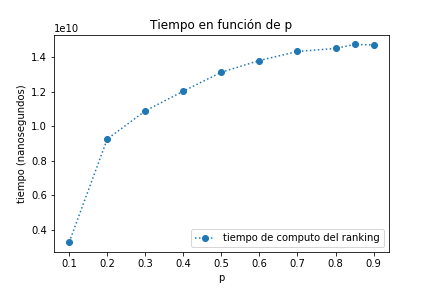
\includegraphics{img/tiempo_p.png} 
  \end{center}
\caption{Tiempo en función de p} \label{fig:exp1-p}
\end{figure}



\newpage

\subsection{Análisis Cualitativo}

\subsubsection{Objetivo:}

En la presente sección se busca analizar la calidad de los rankings calculados por el método de PageRank, evaluarlo según el contexto en el que se lo aplique y relacionándolo con la estructura del grafo subyacente a la red de páginas web a las que deseamos asignarles algún valor de preferencia. \\

Para este fin, diseñamos el siguiente conjunto de instancias. \\

\begin{figure}
   \begin{center}
     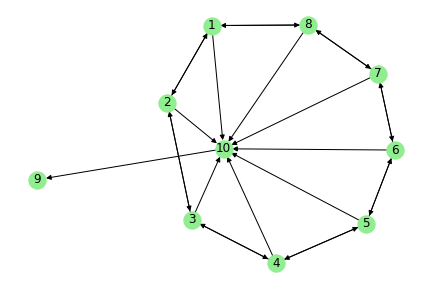
\includegraphics{img/prueba-circular.png} 
  \end{center}
\caption{Grafo 1: Un circuito fuertemente conexo conecta a un nodo y este a otro.} \label{fig:exp3-circular}
\end{figure}

\begin{figure}
   \begin{center}
     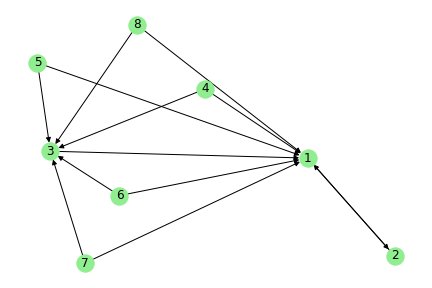
\includegraphics{img/prueba_grafo_2.png} 
  \end{center}
\caption{Grafo 2: Ahora el la página que recibe un link del de mayor grado contiene un link hacia esa} \label{fig:exp3-grafo2}
\end{figure}

\begin{figure}
   \begin{center}
     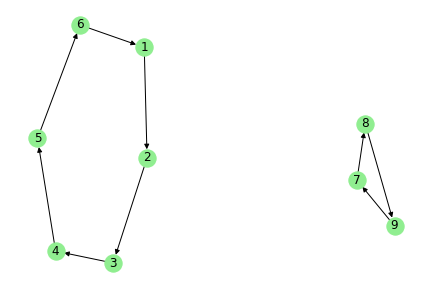
\includegraphics{img/prueba_3_no_conexa.png} 
  \end{center}
\caption{Grafo 3: Grafo de páginas no conexo.} \label{fig:exp3-noconexo}
\end{figure}

\begin{figure}
   \begin{center}
     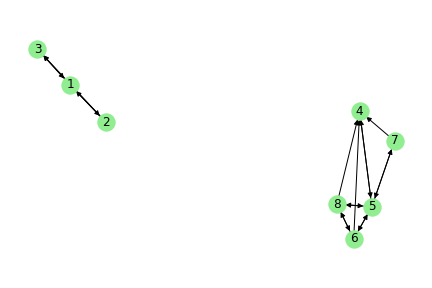
\includegraphics{img/prueba_aislado.png} 
  \end{center}
\caption{Grafo 4: 3 nodos aislados (9,10,11) no se muestran en la ilustración.} \label{fig:exp3-aislado}
\end{figure}

\begin{figure}
   \begin{center}
     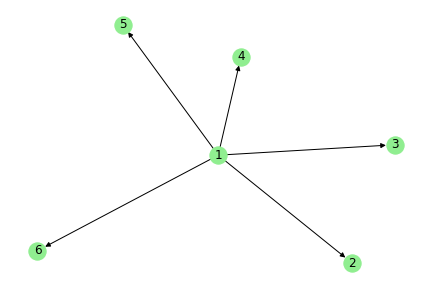
\includegraphics{img/prueba_estrella.png} 
  \end{center}
\caption{Grafo estrella: Una página apunto a todas las demás.} \label{fig:exp3-estrella}
\end{figure}

En el primer grafo, 

\subsubsection{Hipótesis:}

\begin{itemize}
	\item Con respecto al primer grafo, la hipotesis que planteamos es que la página nueve va ser la mas rankeada dado que la página diez es la contiene mas links y ésta sólo tiene un link hacia la página nueve, le está delegando mayor importancia y a su vez la página nueve no tiene links hacia otras páginas, por lo que no reduce su relevancia.
	
\item En el segundo grafo, nuestra hipotesis es que la página uno va ser la mas rankeada ya que la página tres tiene gran importancia y a la única página que referencia es a la uno, además la página uno es referenciada por las mismas páginas que la tres y mas.

\item Para el tercer grafo, la hipotesis plateada es que van a estar todos en el mismo nivel del ranking, es decir, van a estar empatados dado que las páginas son referenciadas y linkeadas por una sola página, lo que haría que todas tuvieran la misma importancia.

\item En el grafo estrella donde todos apuntan a una misma página, este va a ser el de mayor ranking independientemente del p que se elija. 

\Para Por último, para el grafo estrella donde uno apunto a todos, hipotetizamos que que este las páginas que son apuntadas reciben el mismo puntaje y que la página enlazadora arroja un menor puntaje ya que nadie la linkea.  

\end{itemize}

\subsubsection{Resultado y Análisis: }


Los resultados arrojados fueron los siguientes:

\begin{center}
         \begin{tabular}{|c|c|c||c|c|c|}
                    \hline
                    \multicolumn{3}{|c||}{\emph{Ranking} Grafo 1 - \emph{p = 0.3}} & \multicolumn{3}{c|}{\emph{Ranking} Grafo 1 - \emph{p = 0.6}} \\ \hline
                    Pos. & Nodo & Puntaje    & Pos. & Nodo & Puntaje  \\ \hline
1 & 10 & 0.147059 & 1 & 10 &  0.181518 \\ 
2 & 9 & 0.117647 & 2 & 9 &  0.158416 \\
3 & 1 & 0.0919118 & 3 & 1 & 0.0825083 \\
4 & 2 & 0.0919118 & 4 & 2 & 0.0825083 \\
5 & 3 & 0.0919118 & 5 & 3 & 0.0825083 \\
6 & 4 & 0.0919118 & 6 & 4 & 0.0825083 \\
7 & 5 & 0.0919118 & 7 & 5 & 0.0825083 \\
8 & 6 & 0.0919118 & 8 & 6 & 0.0825083 \\
9 & 7 & 0.0919118 & 9 & 7 & 0.0825083 \\
10 & 8 & 0.0919118 & 10 & 8  & 0.0825083 \\ \hline
                    \multicolumn{6}{c}{} \\ \hline
                    \multicolumn{3}{|c||}{\emph{Ranking} Grafo 1 - \emph{p = 0.8}} & \multicolumn{3}{c|}{\emph{Ranking} Grafo 1 - \emph{p = 0.9}} \\ \hline
                    Pos. & Nodo & Puntaje    & Pos. & Nodo & Puntaje  \\ \hline
1 & 10 & 0.197769  & 1 & 9 &  0.212828 \\ 
2 & 9 & 0.193712  & 2 & 10 &  0.204082 \\
3 & 1 & 0.0760649  & 3 & 1 & 0.0728863 \\
4 & 2 & 0.0760649  & 4 & 2 & 0.0728863 \\
5 & 3 & 0.0760649  & 5 & 3 & 0.0728863 \\
6 & 4 & 0.0760649  & 6 & 4 & 0.0728863 \\
7 & 5 & 0.0760649  & 7 & 5 & 0.0728863 \\
8 & 6 & 0.0760649  & 8 & 6 & 0.0728863 \\
9 & 7 & 0.0760649  & 9 & 7 & 0.0728863 \\
10 & 8 & 0.0760649 & 10 & 8  & 0.0728863 \\ \hline

                \end{tabular}
            \end{center}

Grafo 2:

\begin{center}
         \begin{tabular}{|c|c|c||c|c|c|}
                    \hline
                    \multicolumn{3}{|c||}{\emph{Ranking} Grafo 2 - \emph{p = 0.3}} & \multicolumn{3}{c|}{\emph{Ranking} Grafo 2 - \emph{p = 0.6}} \\ \hline
                    Pos. & Nodo & Puntaje    & Pos. & Nodo & Puntaje  \\ \hline
1 & 1 &  0.247596 & 1 & 1 & 0.359375 \\ 
2 & 2 &  0.161779 & 2 & 2 & 0.265625 \\
3 & 3 &  0.153125  & 3 & 3 & 0.125 \\
4 & 4 &  0.0875  & 4 & 4 &  0.05 \\
5 & 5 &  0.0875  & 5 & 5 &  0.05 \\
6 & 6 &  0.0875  & 6 & 6 &  0.05 \\
7 & 7 &  0.0875  & 7 & 7 &  0.05 \\
8 & 8 &  0.0875  & 8 & 8 &  0.05 \\
 \\ \hline
                    \multicolumn{6}{c}{} \\ \hline
                    \multicolumn{3}{|c||}{\emph{Ranking} Grafo 2 - \emph{p = 0.8}} & \multicolumn{3}{c|}{\emph{Ranking} Grafo 2 - \emph{p = 0.9}} \\ \hline
                    Pos. & Nodo & Puntaje    & Pos. & Nodo & Puntaje  \\ \hline
1 & 1 & 0.430556 & 1 & 1 & 0.465461 \\ 
2 & 2 & 0.369444 & 2 & 2 & 0.431414 \\
3 & 3 & 0.075  & 3 & 3 & 0.040625 \\
4 & 4 & 0.025  & 4 & 4 & 0.0125 \\
5 & 5 & 0.025  & 5 & 5 & 0.0125 \\
6 & 6 & 0.025  & 6 & 6 & 0.0125 \\
7 & 7 & 0.025  & 7 & 7 & 0.0125 \\
8 & 8 & 0.025  & 8 & 8 & 0.0125 \\

 \\ \hline

                \end{tabular}
            \end{center}
            
Grafo 3: 

\begin{center}
         \begin{tabular}{|c|c|c|}
                    \hline
                    \multicolumn{3}{|c||}{\emph{Ranking} Grafo 3 - \emph{p = 0.3, 0.6, 0.8, 0.9}} \\ \hline
Pos. & Nodo & Puntaje \\ \hline
1 & 1 & 0.111111 \\ 
2 & 2 & 0.111111 \\
3 & 3 & 0.111111 \\
4 & 4 & 0.111111 \\
5 & 5 & 0.111111  \\
6 & 6 & 0.111111  \\
7 & 7 & 0.111111   \\
8 & 8 & 0.111111 \\
9 & 9 & 0.111111  \\
 \hline

                \end{tabular}
            \end{center}
            
Grafo 4 con aislados:

\begin{center}
         \begin{tabular}{|c|c|c||c|c|c|}
                    \hline
                    \multicolumn{3}{|c||}{\emph{Ranking} Grafo 4 - \emph{p = 0.3}} & \multicolumn{3}{c|}{\emph{Ranking} Grafo 4 - \emph{p = 0.6}} \\ \hline
                    Pos. & Nodo & Puntaje    & Pos. & Nodo & Puntaje  \\ \hline
1 & 5 & 0.131359 & 1 & 5 & 0.174397 \\ 
2 & 1 & 0.111924 & 2 & 1 & 0.133779 \\
3 & 4 & 0.108624  & 3 & 4 & 0.125348 \\
4 & 3 & 0.0990099  & 4 & 3 & 0.108696 \\
5 &  6 & 0.0879543 & 5 & 6 & 0.0870474 \\
6 & 8 & 0.0879543  & 6 & 8 & 0.0870474 \\
7 & 2 & 0.0860956  & 7 & 2 & 0.083612 \\
8 &  7 & 0.0791588 & 8 & 7 & 0.0696379 \\
9 &  9 & 0.0693069 & 9 & 9 & 0.0434783 \\
10 & 10 & 0.0693069  & 10 & 10 & 0.0434783\\
11 & 11 & 0.0693069  & 11 & 11 & 0.0434783 \\ \hline
                    \multicolumn{6}{c}{} \\ \hline
                    \multicolumn{3}{|c||}{\emph{Ranking} Grafo 4 - \emph{p = 0.8}} & \multicolumn{3}{c|}{\emph{Ranking} Grafo 4 - \emph{p = 0.9}} \\ \hline
                    Pos. & Nodo & Puntaje    & Pos. & Nodo & Puntaje  \\ \hline
1 & 5 & 0.205095 & 1 & 5 & 0.221261 \\ 
2 & 1 & 0.149502 & 2 & 1 & 0.157873 \\
3 & 4 & 0.13673  & 3 & 4 & 0.142655 \\
4 & 3 & 0.116279  & 4 & 3 & 0.120482 \\
5 &  6 & 0.0876475 & 5 & 6 & 0.0883312 \\
6 & 8 & 0.0876475 & 6 & 8 & 0.0883312 \\
7 & 2 & 0.0830565  & 7 & 2 & 0.083091 \\
8 &  7 & 0.0642749 & 8 & 7 & 0.0618318 \\
9 &  9 & 0.0232558& 9 & 9 & 0.0120482 \\
10 & 10 & 0.0232558  & 10 & 10 & 0.0120482\\
11 & 11 & 0.0232558  & 11 & 11 & 0.0120482 \\ \hline

                \end{tabular}
            \end{center}
            
Grafo Estrella Saliente:

\begin{center}
         \begin{tabular}{|c|c|c||c|c|c|}
                    \hline
                    \multicolumn{3}{|c||}{\emph{Ranking} Grafo Estrella - \emph{p = 0.3}} & \multicolumn{3}{c|}{\emph{Ranking} Grafo Estrella - \emph{p = 0.6}} \\ \hline
                    Pos. & Nodo & Puntaje    & Pos. & Nodo & Puntaje  \\ \hline
1 & 2 & 0.168254 & 1 & 2 & 0.169697 \\ 
2 & 3 & 0.168254 & 2 & 3 & 0.169697 \\
3 & 4 & 0.168254  & 3 & 4 & 0.169697 \\
4 & 5 & 0.168254  & 4 & 5 & 0.169697 \\
5 &  6 & 0.168254 & 5 & 6 &  0.169697 \\
6 & 1 & 0 0.15873 & 6 & 1 &  0.151515 \\ \hline
                    \multicolumn{6}{c}{} \\ \hline
                    \multicolumn{3}{|c||}{\emph{Ranking} Grafo Estrella - \emph{p = 0.8}} & \multicolumn{3}{c|}{\emph{Ranking} Grafo Estrella - \emph{p = 0.9}} \\ \hline
                    Pos. & Nodo & Puntaje    & Pos. & Nodo & Puntaje  \\ \hline
1 & 2 & 0.170588 & 1 & 2 & 0.171014 \\ 
2 & 3 & 0.170588 & 2 & 3 & 0.171014 \\
3 & 4 & 0.170588  & 3 & 4 & 0.171014 \\
4 & 5 & 0.170588  & 4 & 5 & 0.171014 \\
5 &  6 & 0.170588 & 5 & 6 &  0.171014 \\
6 & 1 & 00.147059 & 6 & 1 &  0.144928 \\ \hline

                \end{tabular}
            \end{center}
            
Grafo Estrella Entrante:

\begin{center}
         \begin{tabular}{|c|c|c||c|c|c|}
                    \hline
                    \multicolumn{3}{|c||}{\emph{Ranking} Grafo Estrella Entrante - \emph{p = 0.3}} & \multicolumn{3}{c|}{\emph{Ranking} Grafo Estrella entrante - \emph{p = 0.9}} \\ \hline
                    Pos. & Nodo & Puntaje    & Pos. & Nodo & Puntaje  \\ \hline
1 & 1 & 0.333333 & 1 & 1 & 0.52381 \\ 
2 & 2 & 0.133333 & 2 & 2 & 0.0952381 \\
3 & 3 & 0.133333  & 3 & 3 & 0.0952381 \\
4 & 4 & 0.133333  & 4 & 4 & 0.0952381 \\
5 &  5 & 0.133333 & 5 & 5 &  0.0952381\\
6 & 6 & 0.133333 & 6 & 6 & 0.0952381 \\
 \hline
                    \multicolumn{3}{c}{} \\ \hline
                    \multicolumn{3}{|c||}{\emph{Ranking} Grafo estrella 1 eje - \emph{p = 0.3}} & \multicolumn{3}{c|}{\emph{Ranking} Grafo estrella entrante 1 eje - \emph{p = 0.9}} \\ \hline
                    Pos. & Nodo & Puntaje    & Pos. & Nodo & Puntaje  \\ \hline
1 & 1 & 0.320513 & 1 & 1 & 0.482456 \\ 
2 & 6 & 0.212821 & 2 & 6 &  0.450877 \\
3 & 2 & 0.116667  & 3 & 2 & 0.0166667 \\
4 & 3 & 0.116667  & 4 & 3 & 0.0166667 \\
5 &  4 & 0.116667 & 5 & 4 &  0.0166667 \\
6 & 5 & 0.116667 & 6 & 5 & 0.0166667 \\
 \hline
 
                    \multicolumn{3}{c}{} \\ \hline
                    \multicolumn{3}{|c||}{\emph{Ranking} Grafo estrella 2 ejes - \emph{p = 0.3}} & \multicolumn{3}{c|}{\emph{Ranking} Grafo estrella entrante 2 ejes - \emph{p = 0.9}} \\ \hline
                    Pos. & Nodo & Puntaje    & Pos. & Nodo & Puntaje  \\ \hline 
 1 & 1 & 0.320513 & 1 & 1 & 0.482456 \\ 
2 & 5 & 0.164744 & 2 & 6 &  0.233772 \\
3 & 6 & 0.164744  & 3 & 2 &  0.233772 \\
4 & 2 & 0.116667  & 4 & 3 & 0.0166667 \\
5 &  3 & 0.116667 & 5 & 4 &  0.0166667 \\
6 & 4 & 0.116667 & 6 & 5 & 0.0166667 \\ \hline

                    \multicolumn{3}{c}{} \\ \hline
                    \multicolumn{3}{|c||}{\emph{Ranking} Grafo estrella 3 ejes - \emph{p = 0.3}} & \multicolumn{3}{c|}{\emph{Ranking} Grafo estrella entrante 3 ejes - \emph{p = 0.9}} \\ \hline
                    Pos. & Nodo & Puntaje    & Pos. & Nodo & Puntaje  \\ \hline 


1 & 1 & 0.320513 & 1 & 1 & 0.482456 \\ 
2 & 4 & 0.148718 & 2 & 4 &  0.161404 \\
3 & 5 & 0.148718  & 3 & 5 &  0.161404 \\
4 & 6 & 0.148718  & 4 & 6 &  0.161404 \\
5 & 2 & 0.116667 & 5 & 2 &  0.0166667 \\
6 & 3 & 0.116667 & 6 & 3 & 0.0166667 \\ \hline

                    \multicolumn{3}{c}{} \\ \hline
                    \multicolumn{3}{|c||}{\emph{Ranking} Grafo estrella 4 ejes - \emph{p = 0.3}} & \multicolumn{3}{c|}{\emph{Ranking} Grafo estrella entrante 4 ejes - \emph{p = 0.9}} \\ \hline
                    Pos. & Nodo & Puntaje    & Pos. & Nodo & Puntaje  \\ \hline 

1 & 1 & 0.320513 & 1 & 1 & 0.482456 \\ 
2 & 3 & 0.140705 & 2 & 3 &  0.125219 \\
3 & 4 & 0.140705  & 3 & 4 &  0.125219 \\
4 & 5 & 0.140705  & 4 & 5 &  0.125219 \\
5 & 6 & 0.140705 & 5 & 6 &  00.125219 \\
6 & 2 & 0.116667 & 6 & 2 & 0.0166667 \\ \hline

                    \multicolumn{3}{c}{} \\ \hline
                    \multicolumn{3}{|c||}{\emph{Ranking} Grafo estrella 5 ejes - \emph{p = 0.3}} & \multicolumn{3}{c|}{\emph{Ranking} Grafo estrella entrante 5 ejes - \emph{p = 0.9}} \\ \hline
                    Pos. & Nodo & Puntaje    & Pos. & Nodo & Puntaje  \\ \hline 

1 & 1 & 0.320513 & 1 & 1 & 0.482456 \\ 
2 & 2 & 0.135897 & 2 & 2 &  0.103509 \\
3 & 3 & 0.135897  & 3 & 3 &  0.103509 \\
4 & 4 & 0.135897  & 4 & 4 &  0.103509 \\
5 & 5 & 0.135897 & 5 & 5 &  00.103509 \\
6 & 6 & 0.135897 & 6 & 6 & 00.103509 \\ \hline

                \end{tabular}
            \end{center} 
            
análisis.            
                                               